
% \section{Benchmarks}
% \subsection{Experiments}
\section{Experiments}\label{sec:experiments}
We establish the compression performance of our selected neural and non-neural compression methods on our proposed datasets.
We describe our experiment protocol in Sec.~\ref{sec:training}, and present our main results in Sec.~\ref{sec:main-results}. Our results show that, even with only minimal architectural adjustments, neural compression can match or even surpass the best classical codecs. 
Our bit-rate estimates obtained with VDM \citep{kingma2021variational} consistently dominate all the neural and non-neural methods considered, suggesting significant room for future improvements.
On the other hand, neural codecs designed for natural image data, such as L3C and PixelCNN, have difficulty exploiting cross-frame correlations in astronomy images, likely due to the image noise characteristics. 

%Overall, the results suggest that in terms of compression ratio, our chosen neural compression methods perform on par with or marginally better than state-of-the-art non-neural methods for 2D image compression, which in turn handily beat classical methods such as Rice.

To better understand how the behavior of the algorithms depends on data characteristics, we examine bit-rate allocation both qualitatively and quantitatively in Sec.~\ref{sec:noise-effect}. Echoing earlier findings from \citet{pence2009lossless}, we see a strong correlation between bit-rate and measures of noise such as SNR and exposure time, confirming that most of the bits are allocated to noisy pixels that can be well modeled by i.i.d. white noise distributions.  Lastly, we explore the out-of-domain generalization performance of a neural compression method, Integer Discrete Flows, in Sec.~\ref{sec:generalization}.

% \subsection{Benchmarks}\label{sec:benchmark-datasets}
% We evaluate neural and traditional compression methods on the following benchmark experiments:

% \begin{enumerate}
%     \item LCO -- 2D image compression experiment on the images from the Las Cumbres Observatory in the GBI-16-2D-Legacy dataset.
%     \item Keck -- 2D image compression experiment on the images from the GBI-16-2D dataset.
%     \item Hubble -- 2D image compression experiment on the images from the SBI-16-2D dataset.
%     \item Webb -- 2D image compression experiment on the images from the GBI-16-3D dataset. Image is the image taken from the first time step in the 3D time-series image tensor.
%     \item SDSS -- 2D image compression experiment on the images from the GBI-16-4D dataset. Image is the image taken from the first time step on the third wavelength band $r$.
%     \item JWST-Res -- 2D image compression experiment on the \textit{residual} image between each time step from the GBI-16-3D dataset. The residual image is obtained by taking the image from the current timestep $t$ minus the image from previous timestep $t-1$. This experiment include residual images from all timesteps. 
%     \item SDSS-3Wave -- 3 channels 2D image compression experiment on the images from the GBI-16-4D dataset.Image is taken from the first timestep on the middle 3 wavelengths $(g, r, i)$.
%     \item SDSS-3Step -- 3 channels 2D image compression experiment on the images from the GBI-16-4D dataset. Image is taken from the first 3 timesteps on the third wavelength band $r$.
% \end{enumerate}

\subsection{Compression Methods}
\label{sec:methods}

We note that astronomy-specific compression implementations have stalled since \citet{pence2009lossless}, and so the latest algorithm in current use is Rice. The most recent works by \citep{maireles2023efficient} and the CCSDS \citep{ccsds2022} have established JPEG-2000 as a state-of-the-art, though it has yet to be deployed to telescopes. Members of our team regularly work with astronomy data collections pipelines, and we confirm this information.

We consider four non-neural methods as baselines, including three standard codecs from the Joint Photographic Experts Group (JPEG) and one codec developed by the Jet Propulsion Laboratory (JPL). The \texttt{imagecodecs} library provides the necessary APIs for all methods. Specifically, we run \textbf{JPEG-XL}, \textbf{JPEG-LS}, \textbf{JPEG-2000}, and \textbf{RICE} codecs in lossless mode with default settings. Additionally, we run JPEG-XL under standard and maximum effort modes as an extra reference, an algorithm that has not been tested for astronomy in any previous works, and show that it establishes a new state-of-the-art amongst non-neural methods. 

We adopt three well-known \textit{practical} neural lossless compression methods in the literature, representing key approaches in deep generative modeling for compression:

\textbf{Integer Discrete Flows (IDF) \citep{hoogeboom2019integer}:} a flow-based model extending the concept of normalizing flows \citep{rezende2015variational} for lossless compression. Unlike conventional normalizing flow models that operate on continuous data, IDF employs discrete bijective mappings using invertible neural networks to connect discrete pixels with a discrete latent.
    
% \textbf{L3C \citep{mentzer2019practical}} is based on learning a hierarchical VAE of the image data, and compresses a given image by first entropy-coding the discrete latent variables, and then entropy-coding the image under the conditional likelihood model given the latents.  

\textbf{L3C \citep{mentzer2019practical}}: a VAE-based lossless compression method utilizing a two-part code \citep{yang2023introduction}. It trains a hierarchical VAE with discrete latents; a given image is compressed by first entropy coding the inferred latents, and then entropy coding the image conditioned on the latents.
% to capture high-level information about the input image.


\textbf{PixelCNN++ \citep{pixelcn}:} an autoregressive model using masked convolutions to model the distribution of each pixel given previous pixels in a raster scan order. 
% The logistic distribution is used for this purpose. 
PixelCNN++ naturally allows for lossless compression using autoregressive entropy coding \citep{mentzer2019practical}.
% employing the predicted distribution of the model for entropy coding on each pixel given previously encoded/decoded pixels \citep{mentzer2019practical}.

Additionally, we use \textbf{Variational Diffusion Model (VDM) \citep{kingma2021variational}} to demonstrate the theoretical performance achievable by current state-of-the-art likelihood-based models. Unlike most diffusion models that target sample quality, VDM incorporates a learned noise schedule and Fourier features, and surpasses Transformer-based autoregressive models on likelihood scores. The likelihood score of VDM can be operationalized as the lossless compression cost of bits-back coding \citep{townsend2019practical, kingma2021variational}, although the resulting codec requires a high number of diffusion steps for encoding/decoding and may not be practical.

\textbf{Handling 16-bit data}: Most neural lossless compression methods are designed for RGB image compression, operating on 8-bit (unsigned) integers. 
% These models compute a categorical probability over the $2^8$ possible discrete values for entropy coding. Extending this to 16-bit symbols, which have $2^{16}$ values, is computationally challenging. To address this, 
To accommodate 16-bit data of AstroCompress, we minimally modify the neural compression methods as follows: for L3C and PixelCNN++, which both use a discretized logistic mixture likelihood model \citep{pixelcn}, we increase the number of bins from $2^8 -1$ to $2^{16}-1$; for IDF, we simply change the input normalization constant from $2^8$ to $2^{16}$. 
Alternatively, we consider treating each 16-bit pixel as two sub-pixels: the most significant byte (MSB) and the least significant byte (LSB), converting a 1-channel 16-bit image into a 2-channel 8-bit image; we then double the number of input channels of each model accordingly. We refer to Supplementary Material for more details.

% We evaluated compression performance on both image variants and found that this approach did not significantly affect performance for IDF and, in some cases, improved compression compared to using the original 16-bit image.




\subsection{Experiment setup}
\label{sec:training}

% \paragraph{Handling 16-bit data} Most neural lossless compression methods were designed with RGB image compression in mind, and hence operate on 8-bit (unsigned) integers. 
% Most neural lossless compression methods compute a categorical probability over the $2^8=256$ possible discrete values for entropy coding; however naively doing so for 16-bit symbols would amount to $2^{16}$ values, which can be computationally challenging. 
% To investigate the effect of this increased range of pixel values, we treat each 16-bit ``pixel'' as consisting of two sub-pixels containing the most significant byte (MSB) and least significant byte (LSB) of the 16-bits. Doing this converts the original 1-channel 16-bit image to a 2-channel 8-bit image. We evaluate compression performances on both variants of the image by extend these methods to handle 16-bit input. This did not seem to significantly affect the performance for IDF and, in some cases, yielded better compression performance compared to using the original 16-bit image.

% \paragraph{Data Preprocessing} For all experiments, we adhere to a fixed split of training and testing images for model training and evaluation (see Supplement for split details). Within our training set, we further partition the training data into $85/15$ split for train and validation sets respectively. Each model is trained and evaluated on 2 variants of the dataset: 16-bit single channel and 8-bit 2 channels using the conversion described above. We report the best compression performance between both variants for each compression algorithm. During training and validation, we perform data augmentation by taking a random $H \times W$ crop from the original image and applying a horizontal flip with a probability of 50\%. For evaluation, we divide each image evenly into $H \times W$ patches, apply reflective padding beforehand if necessary. We then evaluate the compression performance of the model by evaluating all patches belonging to the same image, combining the compression results of these patches to determine the overall compression performance for that image. This process is repeated for all images in the test set, and the average compression performance across all test images is then reported. Note that the compression performance reported is the negative log-likelihood assigned by the model on the given image, and is closely aligned with actual on-disk entropy coding performance using arithmetic coding.

% \paragraph{Data selection} 
We experiment on two categories of data: single-frame images and spectrally/temporally correlated images captured at multiple wavelengths or time steps. We consider the LCO, Keck, and Hubble datasets as single-frame image datasets. For the JWST datasets, we select the first time step of each 3D image cube and form a single-frame dataset, called JWST-2D, and the residual (i.e., difference) between consecutive frames as a separate, temporally correlated dataset, called JWST-2D-Res.
% In principle, entire JWST 3D arrays could be compressed by encoding the initial frame % and subsequent residual frames separately.
% Maybe say something about why we didn't explore this possibility in this work.
% For the SDSS dataset, we categorize  the data as follows: the first time step of the $r$ filter band forms a 2D image dataset, called SDSS. The first time step of the $g$, $r$, and $i$ filter bands constitute a 3D image dataset, called SDSS $(g, r, i)$. Finally, the first three time steps of the $r$ filter band create a 3D image dataset, called SDSS (Timestep).
We sub-select three benchmark datasets from SDSS as follows: (1) the first time step of the $r$ filter band forms a single-frame dataset, called SDSS-2D; (2) the first time step of the $g$, $r$, and $i$ filter bands constitute a spectrally correlated dataset, called SDSS-3D$\lambda$; and (3) the first three time steps of the $r$ filter band create a temporally correlated dataset, called SDSS-3DT.

%For the JWST and SDSS datasets, we use them either as standalone 2D or 3D data. 
% Detailed information is provided in Table~\ref{tab:compression_ratio}.


% \paragraph{Data Preprocessing} 
For all experiments, we use a fixed split of training and testing images (details in Supplement). The training set is further divided into 85\% for training and 15\% for validation. 
For each method, we train and evaluate two model variants as described above, either handling 16-bit input directly or treating it as 8-bit input with double the number of channels; we report the best compression performance between the two variants.
% Each model is trained and evaluated on 2 variants of the dataset, either receiving 16-bit single channel and 8-bit 2 channels using the conversion described above. 
% We report the best compression performance between both variants for each compression algorithm. 
% During training and validation, we perform data augmentation by randomly cropping an $H \times W$ patch from the original image and randomly apply a horizontal flip to the patch. 
We train on random $32 \times 32$ spatial patches and apply random horizontal flipping.
For evaluation, we divide each image evenly into % $H \times W$
$32 \times 32$ patches, apply reflective padding beforehand if needed. We evaluate the model's compression performance by compressing all patches of an image and combining the results to determine overall performance on that image. This process is then repeated for all test images, and the average compression performance is reported. Compression ratio is calculated as the uncompressed bit depth / negative log-likelihood assigned by the model, aligning closely with actual on-disk entropy coding performance using arithmetic coding.

\begin{table}[t]
  \centering
  \scriptsize
  % \setlength{\tabcolsep}{2pt}
  \begin{tabular}{@{}c|cccc|ccccc@{}}
    \toprule
    \multirow{2}{*}{\textbf{Experiment}} & \multicolumn{4}{c|}{Neural Methods} & \multicolumn{5}{c}{Non-neural Methods}\\
    \cmidrule(lr){2-10}
    & IDF & L3C & PixelCNN++ & VDM & JPEG-XL (max) & JPEG-XL & JPEG-LS & JPEG-2000 & RICE\\
    \midrule
    LCO & 2.83 & 1.67 & 2.02 & \textbf{3.64} & \underline{2.98} & 2.78 & 2.81 & 2.80 & 2.65 \\
    \midrule
    Keck & 2.04 & 1.89 & \underline{2.08} & \textbf{2.11} & 2.01 & 1.97 & 1.97 & 1.96 & 1.84 \\
    \midrule
    Hubble & 2.94 & 2.90 & 3.13 & \textbf{3.33} & \underline{3.26} & 2.92 & 2.86 & 2.67 & 2.64 \\
    \midrule
    JWST-2D & \textbf{1.44} & \underline{1.38} & \textbf{1.44} & \textbf{1.44} & \underline{1.38} & 1.33 & 1.35 & 1.37 & 1.24 \\
    \midrule
    SDSS-2D & 2.91 & 2.36 & \underline{3.35} & 3.27 & \textbf{3.38} & 3.14 & 3.16 & 3.20 & 2.96 \\
    \bottomrule
    \toprule
    JWST-2D-Res & 3.14 & 2.91 & 2.80 & --- & \textbf{3.35} & 2.37 & \underline{3.24} & 1.69 & 3.08\\
    \midrule
    SDSS-3D$\lambda$ & 3.05 & 2.29 & 2.88 & --- & \textbf{3.49} & 3.23 & 3.24 & \underline{3.28} & 3.05 \\
    \midrule
    SDSS-3DT & 3.03 & 2.59 & 3.02 & --- & \textbf{3.48} & 3.23 & 3.24 & \underline{3.29} & 3.05 \\
    \bottomrule
  \end{tabular}
  
  % \caption{\vspace{0.05cm}Compression ratios for all methods across experiments, with bold text indicating the best performance and underlined text indicating the second best. The top five experiments involve 2D image inputs. The bottom three experiments incorporate additional data dimensions: in JWST (Residual), we compress the residuals between adjacent frames; in SDSS $(g, r, i)$, we select the first frame from three bands $(g, r, i)$; and in SDSS (Timestep), we select the initial three frames from the $r$ band. JPEG-XL (max) indicates the maximum compression ratio setting. For PixelCNN++, we report the result with adaptive online learning in the parentheses.}
  \caption{\vspace{0.05cm}Compression ratios for all methods across experiments, with bold text indicating the best performance and underlined text indicating the second best.
  The top and bottom subsections of the table contain single-frame and spectrally/temporally correlated-frame compression results, respectively. %requires computation is currently not a practical codec, due to runtime requirements.
  }
  \label{tab:compression_ratio}
\end{table}

\subsection{Compression Performance}\label{sec:main-results}

The top subsection of Table \ref{tab:compression_ratio} presents compression ratios on single-frame compression experiments. 
Among the neural codecs, PixelCNN++ and IDF consistently achieve the most competitive performance. The estimated compression performance of VDM significantly surpass all existing methods on most datasets, suggesting significant room for future improvement with neural compression methods.
% . Although lossless compression with VDM is impractically slow, the results suggest significant room for future improvement with neural compression methods.
% VDM represents a significant new state-of-the-art, surpassing all other codecs on LCO by a staggering $22\%$, and on Keck by an impressive $5\%$. However, our implementation is too slow to be practical. 
Among the non-neural codecs, JPEG-XL (max) dominates across all datasets, establishing itself as the new state-of-the-art non-neural method which has not been considered in prior literature. Note that on the LCO dataset, the previous highest compression ratio was 2.79 by \citet{maireles2023efficient}, and our results for JPEG-LS, JPEG-2000, and RICE, are consistent with those of \citet{maireles2023efficient} on this dataset.


% Among practical codecs, PixelCNN++ frequently achieves the best performance, except on the LCO dataset \citep{maireles2022analysis} where it overfits on the small amount of data—whereas IDF thrives.
% This is expected due to its pixel-level autoregressiveness. 
% PixelCNN++ often closely matches JPEG-XL (max) with less than a 4\% difference and occasionally outperforms JPEG-XL with $\sim4$-$10\%$ improvements. IDF also demonstrates competitive performance on many datasets, despite being non-autoregressive. 
% However, JPEG-XL (max) consistently exhibits high compression ratios across datasets.

% Notably, the highest compression ratio previously achieved for the LCO dataset was 2.79 by \citet{maireles2023efficient}, which is noticeably surpassed by VDM and JPEG-XL (max) in our benchmark. Our results for non-neural codecs, including JPEG-LS, JPEG-2000, and RICE, are consistent with the previously published benchmarks \citet{maireles2023efficient} on this dataset.

When it comes to spectrally/temporally correlated data, we expect higher compression ratios for all the methods due to the additional correlations that can be exploited. This is indeed the case, as seen in the bottom subsection of Table \ref{tab:compression_ratio}; however, non-neural codecs show surprisingly superior performance boosts than the neural codecs.
% interestingly non-neural codecs show superior performance boosts on our spectrally/temporally correlated data, as seen in the bottom subsection of Table \ref{tab:compression_ratio}. Neural codecs seem to struggle with capturing correlations across different frames. 
This indicates a need for further improvement in the neural compression techniques, which have largely been designed for image compression, to better extract cross-wavelength or cross-timestep information.
% \textcolor{blue}{One direction of improvement is an adaptive technique for PixelCNN++ on 3D SDSS. By using a pre-trained model on 2D SDSS and sequentially updating the model we obtained performances better than other neural codecs and more than 36\% improvement BPD to the native 3D model with compression ratios of 3.13 and 3.33 for SDSS multi wavelength and time channels respectively. Part of the reason for the improvement is the switch from 8-bit data to 16-bit. 16 bit for 3D PixelCNN++ is not native to the model architecture \citep{pixelcn} hence the performance improvement.}
% \TODO{To be improved by someone(Yibo/Peter): The PixelCNN++ model for 3D SDSS data shows a significantly worse compression ratio than the pretrained 2D SDSS model, suggesting suboptimal convergence. To address this challenge, we are considering an extension of PixelCNN++. For instance, we are exploring an online adaptive learning technique that updates the model pretrained on 2D data as it sequentially compresses inputs along the additional axis dimension.  Initial experiments showed a $\sim50\%$ improvement in compressing the 3D SDSS dataset.}



% \TODO{To be improved by someone(Yibo/Peter): It's worth noting that the PixelCNN++ model tailored for 3D SDSS data shows a significantly worse compression ratio compared to directly using a pretrained 2D SDSS model. This suggests that the models may be converging to suboptimal solutions. To address this challenge, we are considering an extension of PixelCNN++. For instance, we are exploring an online adaptive learning technique that updates the model pretrained on 2D data as it sequentially compresses inputs along the additional axis dimension. Our initial experiments demonstrated a $\approx 50\%$ improvement over the PixelCNN++ in compressing the 3D SDSS dataset.}
% We also notice that the PixelCNN++ often approximately matches JPEG-XL (max) with $<4\%$ difference and sometimes beats JPEG-XL with $4-10\%$ improvements. The greatest improvement is seen in the Keck experiment with the worst performance comparison being (aside from LCO) the Hubble experiment. 
% \textcolor{red}{[TODO @Yibo elaborate on 3-d data?]} For dynamic One-Shot Online model of PixelCNN++ for 3D SDSS datasets, this technique achieved a $~2-3\%$ improvement in compression ratio bringing it to $3.13$ as opposed to $3.07$ without the dynamic updating. For 3D experiments, IDF comes on top within the neural methods but does not show improvements over non-neural methods. 

\sidecaptionvpos{figure}{c}
\begin{SCfigure}[0.75][t]
    \centering
    \includegraphics[width=0.42\textwidth]{figs/hubble_exposure_time.png}
    \caption{Hubble exposure times plotted against compression ratios using various algorithms. Longer exposure times tend to induce more incompressible noise and, hence, reduce compression ratios.}
    \label{fig:exposure_vs_compression}
    \vspace{-1em}
\end{SCfigure}

\subsection{The Effect of Noise}
\label{sec:noise-effect}


% \begin{wrapfigure}{r}{0.5\textwidth}
%     \centering
%     \includegraphics[width=0.5\textwidth]{figs/hubble_exposure_time.png}
%     \caption{Hubble exposure times plotted against compression ratios using various algorithms. Longer exposure times tend to induce more incompressible noise and, hence, reduce compression ratios.}
%     \label{fig:exposure_vs_compression}
%     \vspace{-1em}
% \end{wrapfigure}


\begin{figure}[t]
    \centering
    \includegraphics[width=\textwidth]{figs/bitrate_maps.png}
    \caption{
   From left to right, an example SDSS-2D image: raw image, SNR heatmap, and PixelCNN++ bitrate heatmap. Colors are z-score normalized for visualization; colorbars indicate true values.
   %From left to right, of an example 800x800 SDSS image: raw image, SNR, Pixel-CNN bitrate heatmap. Colors were z-score normalized for visualization; colorbars represent true values.
    }
    \label{fig:bitrate_heatmap}
    \vspace{-1em}
\end{figure}

% \begin{figure}[h]
%     \centering
%     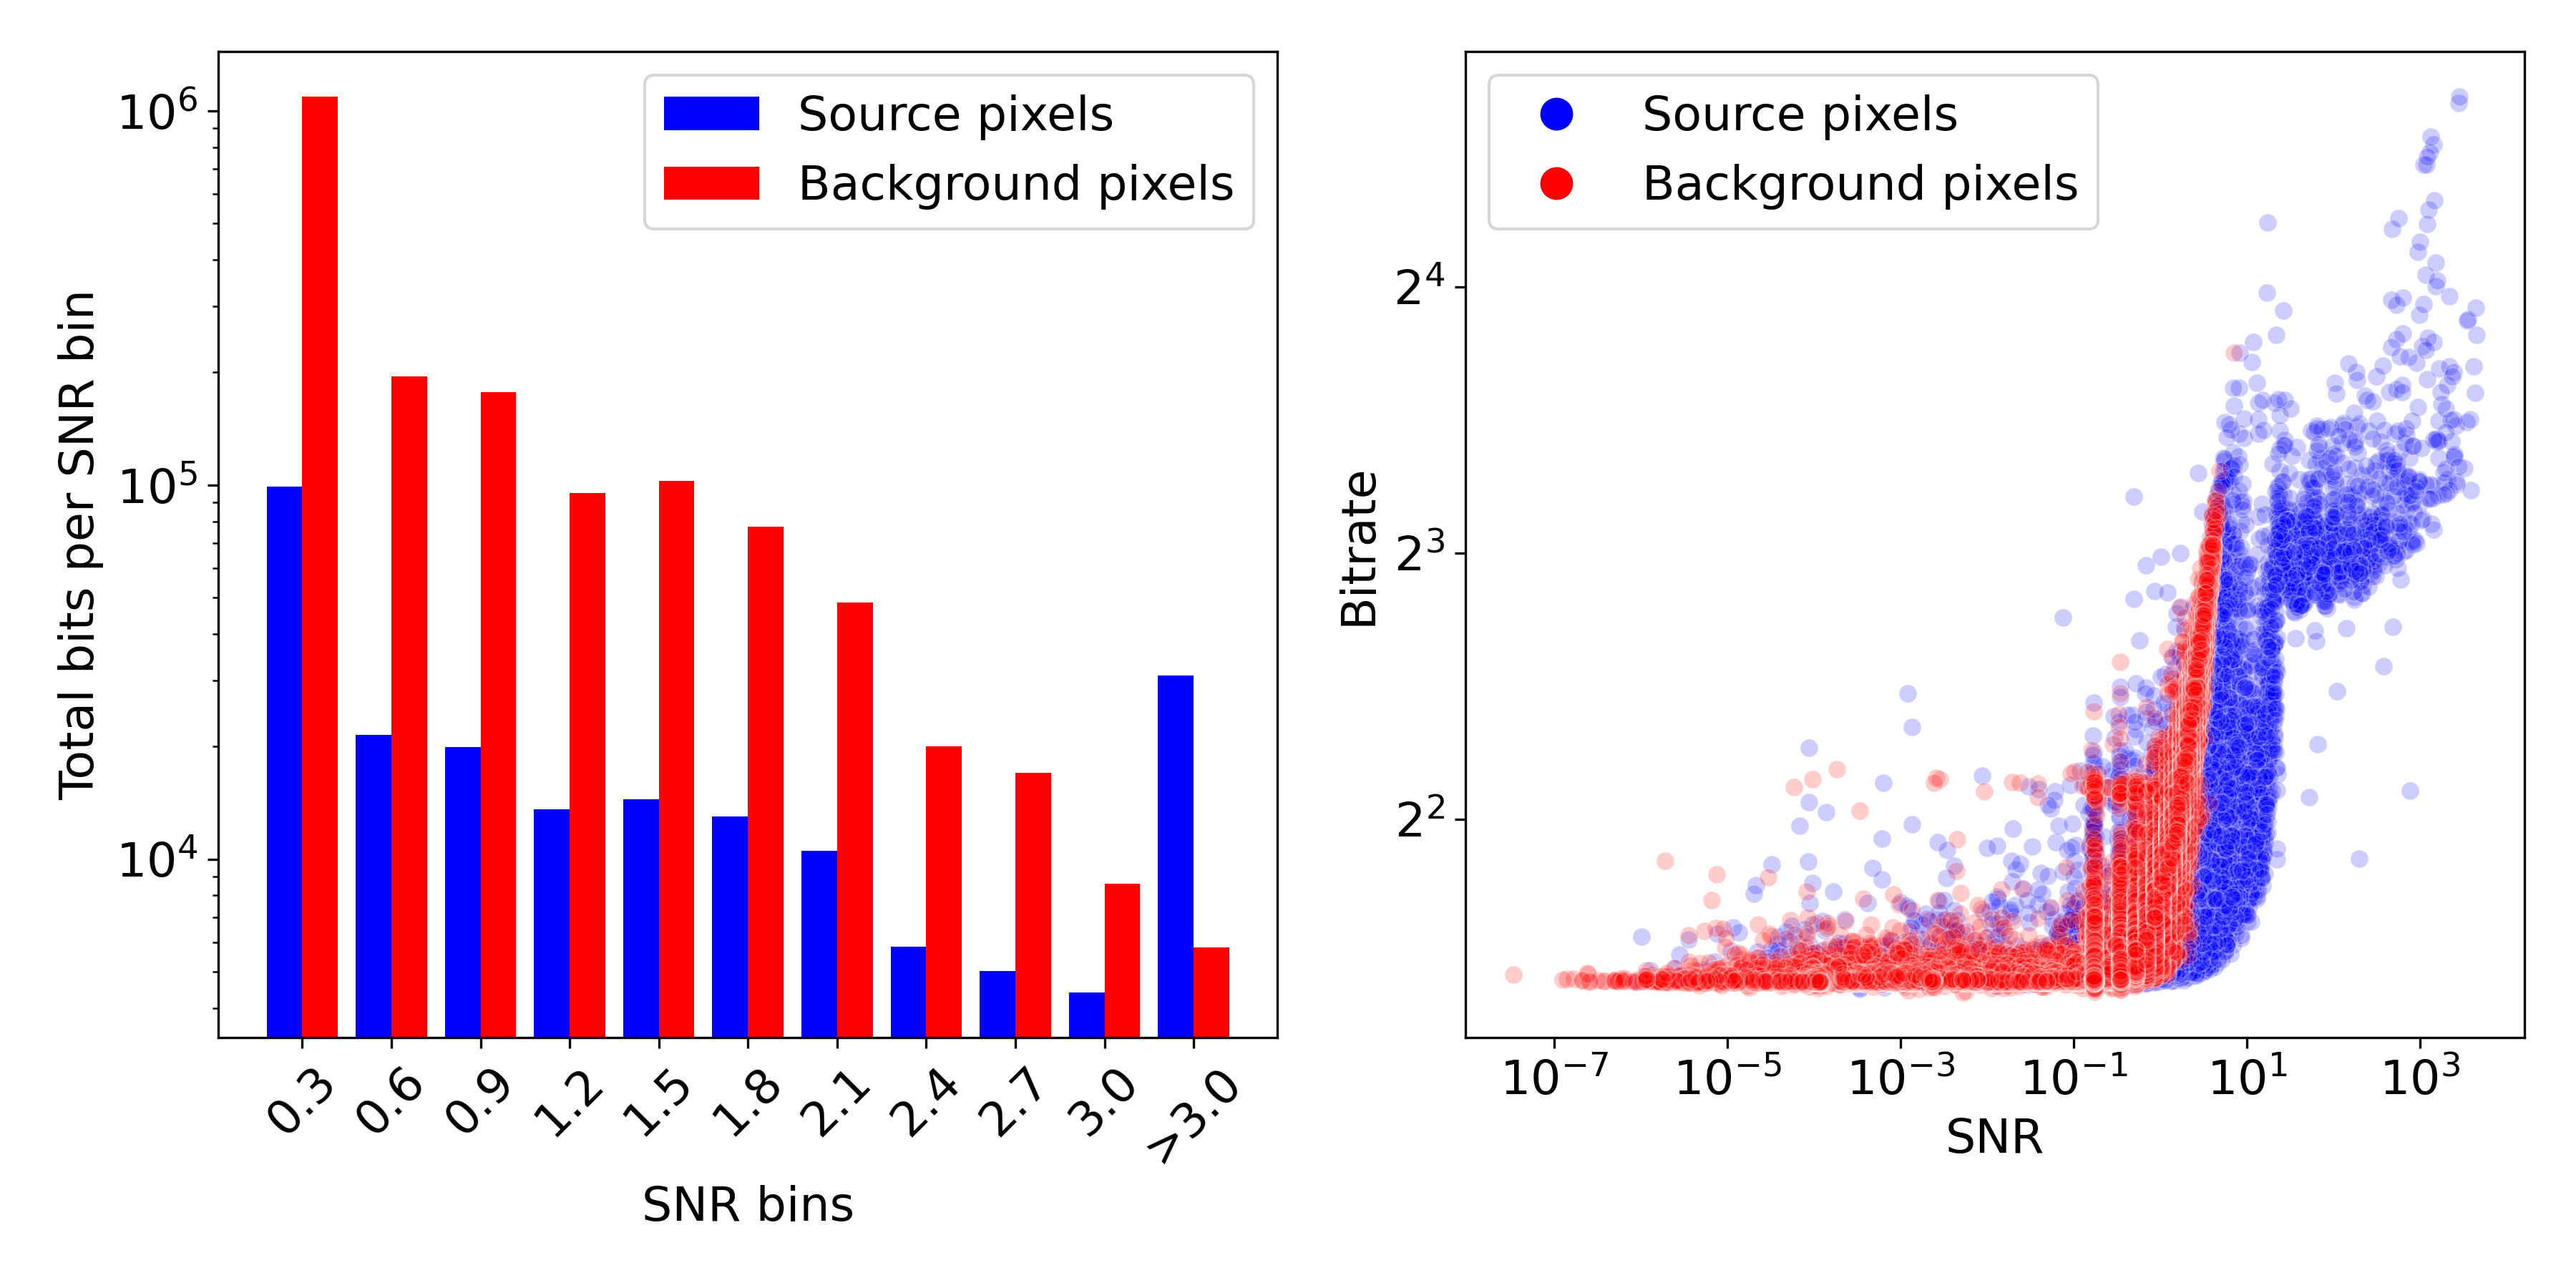
\includegraphics[width=1\textwidth]{figs/histo_and_scatter.png}
%     \caption{Left: histogram demonstrating the bit allocation of PixelCNN++ compression at various SNR values. Right: scatterplot demonstrating the upward correlation of SNR and PixelCNN++ bitrate. The Figure \ref{fig:bitrate_heatmap} image was used here.}
%     \label{fig:bit_allocation}
% \end{figure}


Following \citet{pence2009lossless}, our Figure \ref{fig:exposure_vs_compression} illustrates an inverse relationship between compression ratios and exposure time, which is one of the key variables in determining the signal-to-noise ratio (SNR) in an image. We demonstrate a negative correlation between these two variables, likely because an increase in exposure time results in an increased number of noise bits. We hypothesize that the plateau seen will reverse at higher exposure times as many CCD pixels reach their max physical value, reducing image entropy. In Supplementary Section \ref{sec:additional-data-explorations}, we further explore a strong relationship between background pixel noise levels and compressibility amongst all test images from all datasets.

% For the following figures, we computed a mask of all sources followed by an estimation of the sky's background noise in order to estimate SNR at each pixel using \texttt{\href{https://photutils.readthedocs.io/en/stable/background.html}{photutils}}. The 2D background was estimated by breaking the larger $800$ by $800$ image into $50$ by $50$ patches, then iteratively excluding any pixels above $3\sigma$ of the median value. The medians and standard deviations of each box's remaining pixels are interpolated to the full image size to retrieve the final background and noise images. SNR is then calculated as 
% \texttt{SNR = (original\_image - background) / noise}.
% } Finally, source pixels were detected by applying a kernel around any pixels above $3\sigma$, in order to estimate a smoothed mask around all signal-generating objects. While these figures only represent one image, they are sufficiently representative of the dataset.

Figures \ref{fig:bitrate_heatmap} and \ref{fig:bit_allocation} use data from a single, representative SDSS-2D frame. We used {\texttt{photutils}} \citep{photutils} estimate the sky's background noise to get the SNR at each pixel, and then to compute a mask of all sources. The 2D background was estimated by dividing the $800\times800$ image into $50\times50$ patches and excluding pixels above $3\sigma$ of the median value. The medians and standard deviations of the remaining pixels were interpolated to get the final background and noise images. SNR was calculated as $\texttt{SNR = (original\_image - background) / noise}$. Source pixels were detected by applying a kernel around any pixels above $3\sigma$, creating a smoothed mask for signal-generating objects.

Figure \ref{fig:bitrate_heatmap} demonstrates that source pixels have higher bitrates, as expected—in a sense, these pixels are more "surprising," and thus a lower likelihood is assigned. Interestingly, the background pixel regions of the bitrate heatmap are significantly more noisy than the corresponding SNR background. This suggests that there may be potential for reduction in the bitrate of the higher bitrate background pixels, as we might expect most background pixels to exhaust a similar number of bits.

\begin{figure}[ht]
    \centering
    \begin{minipage}{.2\textwidth}
        \includegraphics[width=1\textwidth]{figs/combined_images_with_aligned_colorbar.png}
        \end{minipage}
    \hfill
    \begin{minipage}{.74\textwidth}
        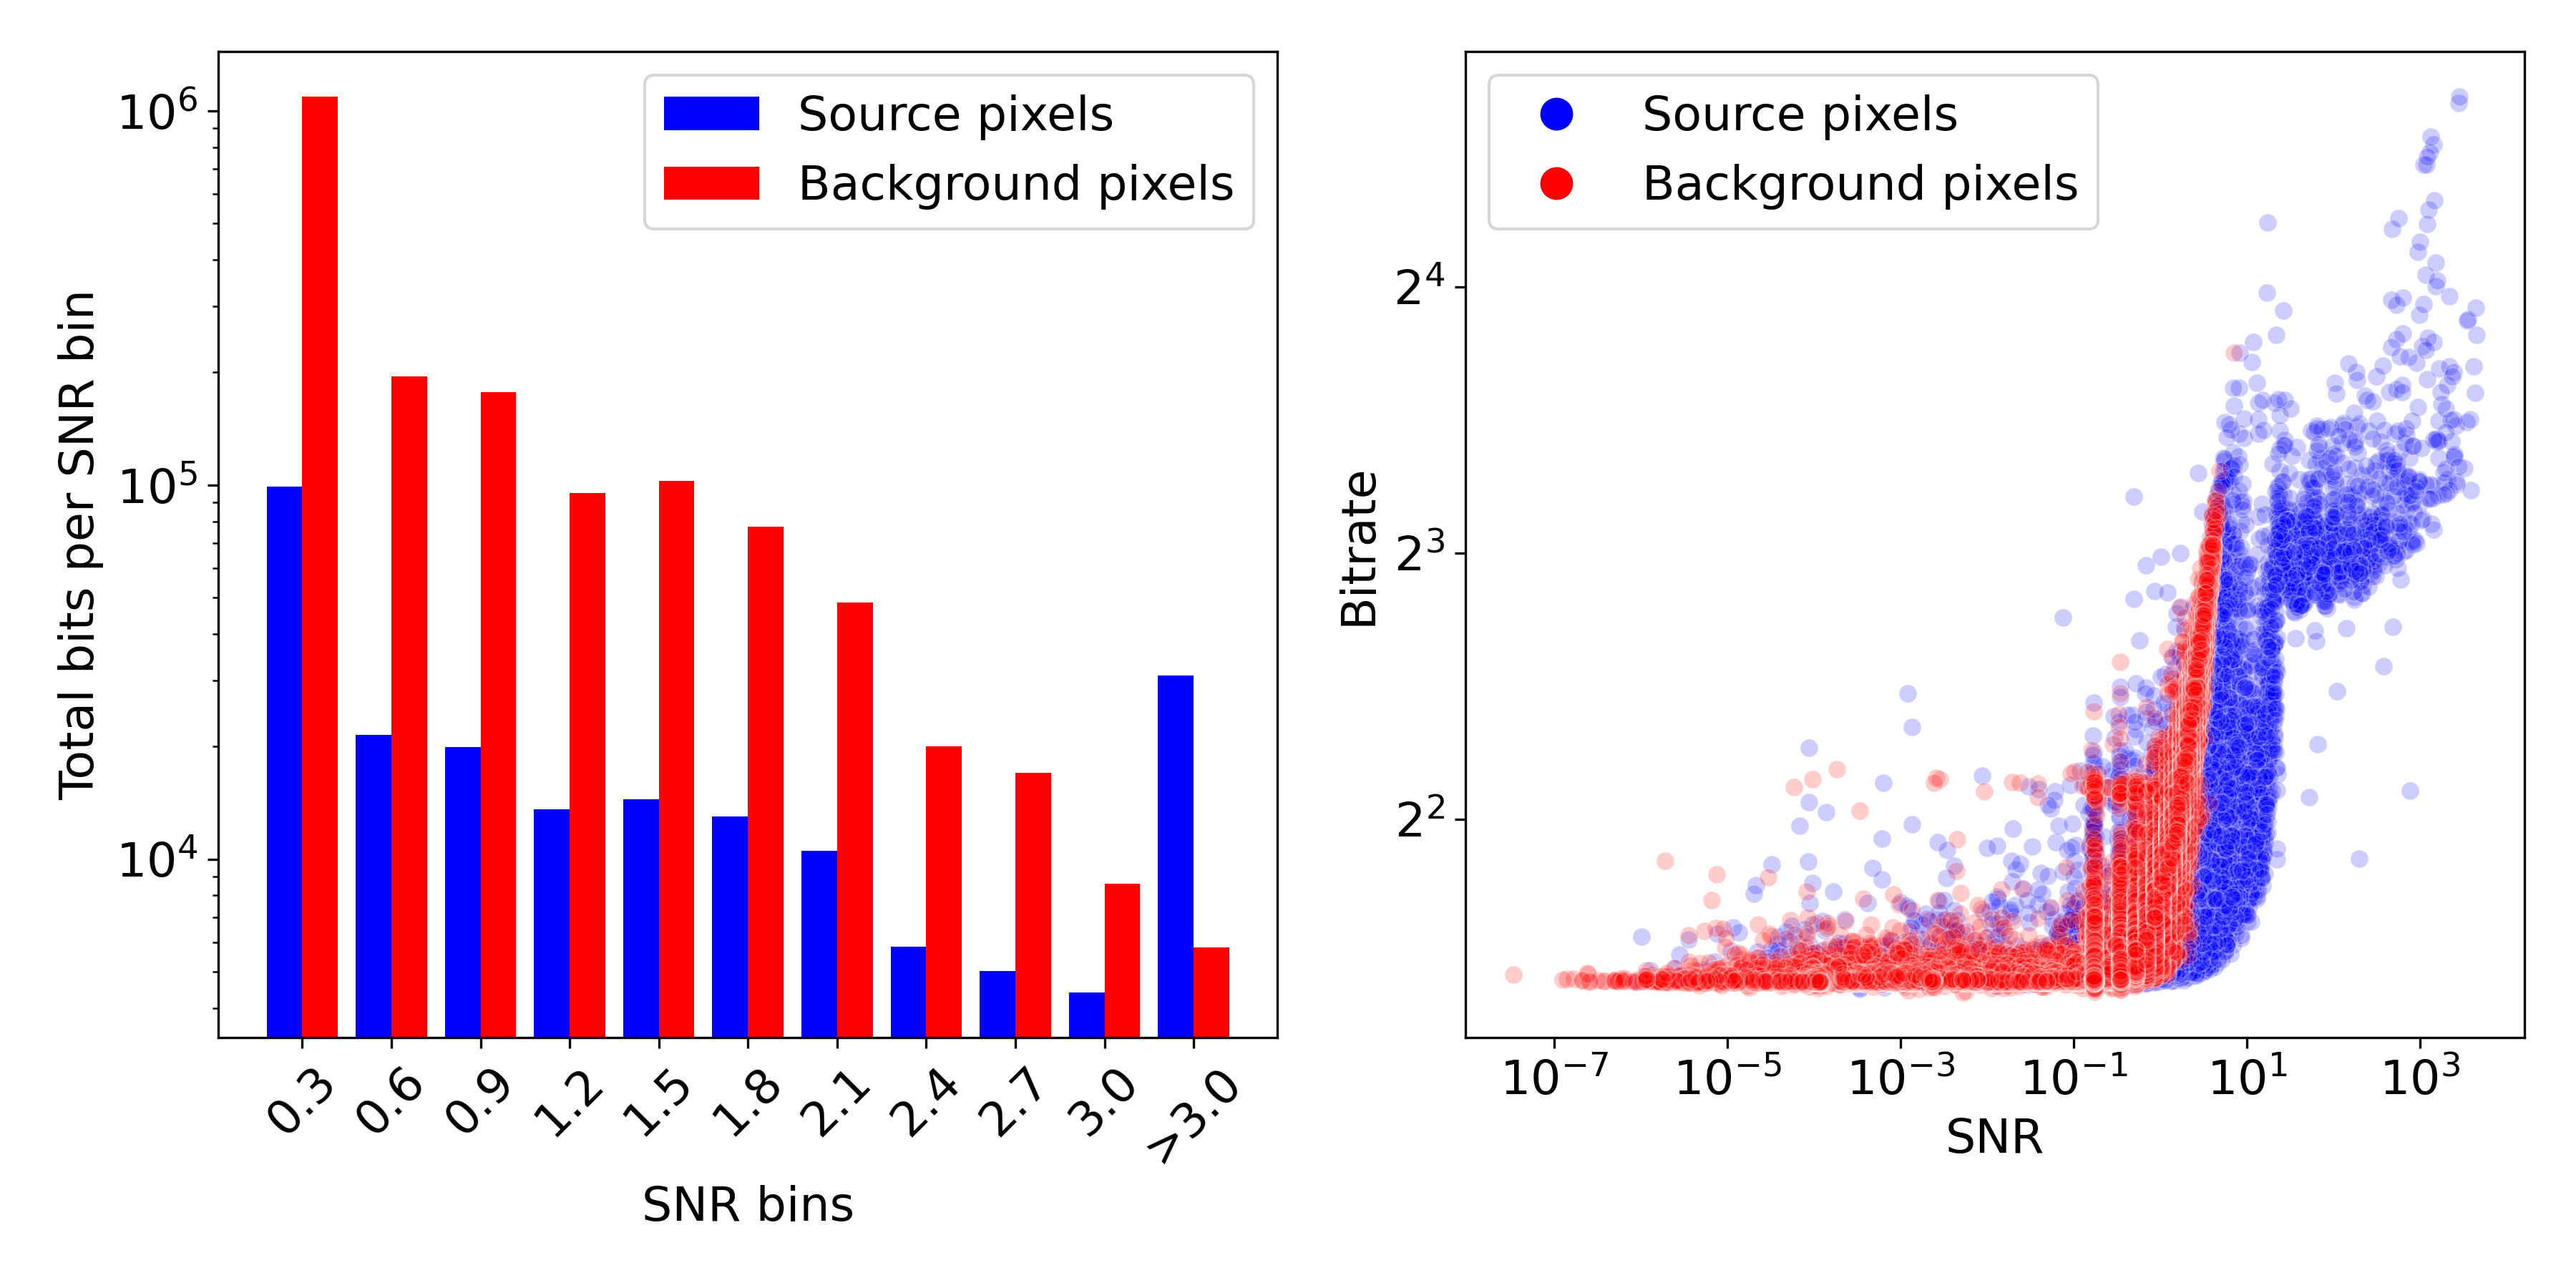
\includegraphics[width=1\textwidth]{figs/histo_and_scatter.png}
        \end{minipage}
    \caption{
    \textbf{Left}: SNR heatmap of an example image (Figure \ref{fig:bitrate_heatmap}), showing source (top) vs. background (bottom) pixels. \textbf{Middle}: histogram of PixelCNN++ total bit allocation for various binned SNR values. \textbf{Right}: scatterplot showing the positive correlation between SNR and PixelCNN++ bitrate.
    %\textbf{Left}: SNR heatmap of an example image corresponding to source (top) v.s. background pixels. \textbf{Middle}: histogram demonstrating the bit allocation of PixelCNN++ compression at various SNR values. \textbf{Right}: scatterplot demonstrating the upward correlation of SNR and PixelCNN++ bitrate. The Figure \ref{fig:bitrate_heatmap} image was used here.
    }
    \label{fig:bit_allocation}
    \vspace{-1em}
\end{figure}

Figure \ref{fig:bit_allocation} furthermore demonstrates the extreme bit-rate consumption by background noise pixels. On this image, $98.5$\% of pixels fell under $3$ SNR. Some source pixels were placed in the lowest SNR bin, but this is likely due to some overestimation of source radii in the source masking process. Interestingly, the scatterplot resembles a step function, with a jump from $\texttt{Bitrate} \approx 3$ bits per pixel to $\texttt{Bitrate} \approx 10$ bits per pixel at $\texttt{SNR} \approx 10^{1}$—the transition point where stars and galaxies emerge over background noise.


\subsection{Generalization performance}\label{sec:generalization}

\begin{wraptable}[13]{R}{6.5cm}
  \centering
  \vspace{-2.05em}
  \tiny
  % \setlength{\tabcolsep}{2pt}
  \begin{tabular}{@{}c|llllll@{}}
    \toprule
    & LCO & Keck & Hubble & JWST-2D & SDSS-2D\\
    \midrule
    LCO & \textbf{2.83} & 1.01 & 1.09 & 0.84 & 2.31   \\
    \midrule
    Keck & 2.70 & \textbf{2.05} & 2.20 & 1.19 & \underline{3.02} \\
    \midrule
    Hubble & 0.67 & 0.94 & \underline{2.94} & 1.22 & 0.69 \\
    \midrule
    JWST-2D & 1.46 & 1.45 & 1.47 & \textbf{1.44} & 1.50 \\
    \midrule
    SDSS-2D & 2.27 & 1.24 & 1.75 & 1.02 & 2.91 \\
    \midrule
    All data & \underline{2.82} & \underline{1.87} & \textbf{2.98} & \underline{1.38} & \textbf{3.18} \\
    \bottomrule
  \end{tabular}
  \caption{IDF generalized performance across single-frame datasets. Rows indicate train set; columns indicate test set. Bold indicates best in the test set; underline indicates second-best.}
  \label{tab:generalization_performance}
  % \vspace{-2em}
\end{wraptable}

% We take IDF as our representative model for investigating generalization performance across 2D image compression based on its empirical performance across datasets compared to other neural compression methods. 
We take IDF as our representative model for investigating generalization performance, where we train and evaluate on all pairs of the single-frame compression tasks, as well as train on all these datasets combined.
Table \ref{tab:generalization_performance} shows that the cross-data generalization performance depends heavily on the training data used, and training on 
some of the datasets (e.g., Keck, JWST-2D) consistently resulted in better generalization performance than others (LCO, Hubble).
% Keck and JWST-2D worked the best. 
%gave the most consistent out-of-distribution performance.
In particular, the test performance on SDSS-2D when trained on Keck was even better than when trained on SDSS-2D itself. We hypothesize that the diversity of wavelength filters and background noise in the Keck dataset, as mentioned in Section \ref{sec:corpus} and shown in Figure \ref{fig:bkg}, may explain its unexpected generalizability. Overall, the best generalization performance was achieved by training on all the datasets combined, suggesting the importance of exposing the model to a variety of data characteristics. Additional model experiments trained on RGB images and evaluated on our dataset are discussed in the supplementary section \ref{app:rgb_cross_eval}. 
% trained model from the Keck experiment generalizes decently across other experiments, even surpassing the model \emph{trained and evaluated} on SDSS-2D. 
 

\subsection{Computational metrics}

% \begin{table}
%   \centering
%   \begin{minipage}{0.49\linewidth}
%     \centering
%     \tiny
%     \begin{tabular}{@{}c|llllll@{}}
%       \toprule
%       & LCO & Keck & Hubble & JWST & SDSS\\
%       \midrule
%       LCO & \textbf{2.83} & 1.01 & 1.09 & 0.84 & 2.31   \\
%       \midrule
%       Keck & \underline{2.70} & \textbf{2.05} & \underline{2.20} & 1.19 & \textbf{3.02} \\
%       \midrule
%       Hubble & 0.67 & 0.94 & \textbf{2.94} & \underline{1.22} & 0.69 \\
%       \midrule
%       JWST & 1.46 & \underline{1.45} & 1.47 & \textbf{1.44} & 1.50 \\
%       \midrule
%       SDSS & 2.27 & 1.24 & 1.75 & 1.02 & \underline{2.91} \\
%       \bottomrule
%     \end{tabular}
%     \caption{IDF generalized performance across 2D experiments. Rows indicate training dataset; columns indicate test dataset. Boldface indicates best in test set; underline indicates second-best.}
%     \label{tab:generalization_performance}
%   \end{minipage}%
%   \hfill
%   \begin{minipage}{0.49\linewidth}
%     \centering
%     \tiny
%     \begin{tabular}{@{}c|ll@{}}
%       \toprule
%       & Sloan (800x800) & Hubble (4144x2068) \\ 
%       \midrule
%       IDF & 0.42 $\pm$ 0.01 & 6.03 $\pm$ 0.24 \\ 
%       \midrule
%       L3C & 5.18 $\pm$ 1.04 & 73.04 $\pm$ 2.36 \\ 
%       \midrule
%       PixelCNN++ & 1.48 $\pm$ 1.05 & 20.49 $\pm$ 0.18 \\ 
%       \midrule
%       JPEG-XL max & 3.14 $\pm$ 0.14 & 87.76 $\pm$ 13.30 \\ 
%       \midrule
%       JPEG-XL default & 0.06 $\pm$ 0.002 & 0.91 $\pm$ 0.07 \\ 
%       \midrule
%       JPEG-LS & 0.02 $\pm$ 0.0002 & 0.316 $\pm$ 0.04 \\ 
%       \midrule
%       JPEG-2000 & 0.09 $\pm$ 0.003 & 1.76 $\pm$ 0.11\\ 
%       \midrule
%       RICE & 0.008 $\pm$ 0.0002 & 0.12 $\pm$ 0.02 \\ 
%       \bottomrule
%     \end{tabular}
%     \caption{Runtime for each compression method (in seconds) on the Sloan and Hubble datasets. For neural methods, the runtime refers to the model inference time on the entire image. For classical methods, the runtime refers to the time taken to convert images to byte streams.}
%     \label{tab:runtime}
%   \end{minipage}
% \end{table}

To offer practical considerations, we present runtime metrics that would be valuable in assessing the feasibility of these methods for real-world applications. Table \ref{tab:runtime} shows various runtime for inference from neural methods and coding time for classical methods. JPEG-XL with max effort and JPEG-2000 seem to scale quadratically with the number of input pixels, while all other neural and non-neural algorithms scale linearly with the number of input pixels. Note that in order to work with limited GPU memory, our neural methods primarily operate on 32 $\times$ 32 patches, which very likely limits the achievable compression ratio. By comparison, our non-neural baselines always receive full images as input. We stress that the JPEG-XL max algorithm takes nearly 90 seconds for a Hubble image, which would likely be infeasible for practical use given that Hubble collects 15-30 GB of data per day, nearly requiring the entire day for compression alone \citep{nasa2014}. %\textbf{
IDF is roughly 10x faster than JPEG-XL max and often outperforms all non-neural methods other than JPEG-XL max.
While we acknowledge that runtimes are inherently hardware and parallelization-dependent, this work is primarily aimed at inspiring a broader research trajectory towards advanced compression techniques over the coming decade. Consequently, we defer the nuanced practical considerations of space-compatible hardware and runtime optimization to future investigations, noting that all presented algorithms leverage unoptimized reference implementations. We note that the long runtime of VDM is currently impractical due to a large number of expensive neural network evaluations. However, there exists extensive research on speeding up diffusion models by several orders of magnitude \citet{salimans2022progressive} \citet{cao2024survey} \citet{ulhaq2022efficient} \citet{yang2023diffusion}, which can potentially translate their excellent bit-rate estimates into practical compression performance.
% However, it pushes the upper bound of potential compression ratios, confirming that significant improvement is possible. There exists extensive literature on speeding up diffusion models by several orders of magnitude (\citet{salimans2022progressive} \citet{cao2024survey} \citet{ulhaq2022efficient} \citet{yang2023diffusion})}.

% Since neural models split images into $32 \times 32$ patches before encoding, they naturally scale linearly with the number of input pixels and can be parallelized. We note that a GPU implementation also exists for JPEG-2000 at \url{https://developer.nvidia.com/nvjpeg}. 

\begin{wraptable}[18]{R}{6cm}
    \centering
    \tiny
    \vspace{-2em}
    \begin{tabular}{@{}c|ll@{}}
        \toprule
        \textbf{Codec} & \textbf{SDSS-2D (800x800)} & \textbf{Hubble (4144x2068)} \\ 
        \midrule
        IDF & 0.42 $\pm$ 0.01 & 6.03 $\pm$ 0.24 \\ 
        \midrule
        L3C & 5.18 $\pm$ 1.04 & 73.04 $\pm$ 2.36 \\ 
        \midrule
        PixelCNN++ & 1.48 $\pm$ 1.05 & 20.49 $\pm$ 0.18 \\ 
        \midrule
        JPEG-XL max & 3.14 $\pm$ 0.14 & 87.76 $\pm$ 13.30 \\ 
        \midrule
        JPEG-XL default & 0.06 $\pm$ 0.002 & 0.91 $\pm$ 0.07 \\ 
        \midrule
        JPEG-LS & 0.02 $\pm$ 0.0002 & 0.316 $\pm$ 0.04 \\ 
        \midrule
        JPEG-2000 & 0.09 $\pm$ 0.003 & 1.76 $\pm$ 0.11\\ 
        \midrule
        RICE & 0.008 $\pm$ 0.0002 & 0.12 $\pm$ 0.02 \\ 
        \specialrule{1.2pt}{2pt}{2pt}
        VDM & 2301 $\pm$ 229.2 & 33072 $\pm$ 19.8 \\ 
        \bottomrule
    \end{tabular}
    \caption{Compression (encoding) runtime (in sec/image) on the SDSS-2D and Hubble datasets. For neural methods, we measure the time for evaluating the likelihood under the model without entropy coding. % the refers to the model likelihood inference time on the full image, without entropy coding. % For classical methods, the runtime refers to the time taken to encode images.
    }
    \label{tab:runtime}
\end{wraptable}